% SPDX-License-Identifier: AGPL-3.0-only OR LicenseRef-SnapKitty-Opaque-1.0
% Copyright (C) 2026 Ahmad Ali Parr / SnapKitty Research Lab
%
% Full paper grown from paper/sovereign_rh_lock_grounding.tex (kept unchanged).
% Build: cd paper && latexmk -pdf sovereign_rh_lock.tex   (or: tectonic sovereign_rh_lock.tex)
% Figure data: paper/figures/*.tex, written by `sh paper/figures/make_pgf.sh build/ro`.
\documentclass[11pt,letterpaper]{article}

\usepackage[letterpaper,margin=22mm]{geometry}
\usepackage{mathptmx}
\usepackage{amsmath,amssymb,amsthm,mathtools}
\usepackage{booktabs}
\usepackage{tabularx}
\usepackage{xcolor}
\usepackage{tikz}
\usetikzlibrary{arrows.meta,positioning,fit,calc}
\usepackage{pgfplots}
\pgfplotsset{compat=1.18}
\usepackage{hyperref}

\definecolor{primary}{RGB}{22,62,110}
\hypersetup{
    colorlinks=true,
    linkcolor=primary,
    citecolor=primary,
    urlcolor=primary,
    pdftitle={SOVEREIGN-RH-LOCK: A Hybrid Neuro-Symbolic and Formal Verification Architecture for the Connes-Berry-Keating Spectral Program},
    pdfauthor={SOVEREIGN-RH-LOCK Research Engine}
}

\setlength{\parskip}{6pt plus 2pt minus 1pt}

\newtheorem{definition}{Definition}
\newtheorem{remark}{Remark}
\newtheorem{obligation}{Proof Obligation}
\newtheorem{theorem}{Theorem}
\newtheorem{proposition}{Proposition}

\newcommand{\takeaway}[2]{%
  \vspace{6pt}\noindent\colorbox{primary!8}{%
    \parbox{\dimexpr\linewidth-2\fboxsep\relax}{%
      \vspace{3pt}\textbf{\color{primary}#1:}\hspace{0.5em}#2\vspace{3pt}%
    }%
  }\vspace{6pt}%
}
\newcommand{\code}[1]{\texttt{#1}}
\AtBeginDocument{\let\origus\_\renewcommand{\_}{\origus\allowbreak}}
\emergencystretch=3em

\title{\textbf{SOVEREIGN-RH-LOCK: A Hybrid Neuro-Symbolic and Formal Verification Architecture for the Connes--Berry--Keating Spectral Program}}
\author{SOVEREIGN-RH-LOCK Research Engine}
\date{November 2026}

\begin{document}

\maketitle

\begin{abstract}
We present \textsc{Sovereign-RH-Lock}, a modular research architecture designed to investigate the Riemann Hypothesis (RH) through the Connes--Berry--Keating spectral program without conflating numerical coincidence with formal mathematical proof. The system separates conjecture generation, numerical measurement, structural classification, closed-world admission and formal verification into distinct layers, each with its own epistemic boundary. This paper describes the native implementation of that architecture: numerical kernels in Fortran~2008 with quad-precision zeta evaluation, a C23 command-line engine that reproduces the original Python reference byte for byte on 49 of 58 golden cases (the remaining 9 within stated floating-point tolerances), an SWI-Prolog bridge from the OWL~2~DL ontology to Answer Set Programming facts, and a Lean~4 formal layer built against Mathlib. The Fortran kernel recomputes all 511 reference zeros of the oracle with maximum deviation $4.99\times10^{-11}$ from the tabulated values, which are given to ten decimals. Discrete Berry--Keating operators are Hermitian to machine precision but, as we show in closed form and by measurement, their spectra are near-arithmetic progressions with spacing $\approx 2.73$ that do not reproduce the zeros, while the unfolded zero spacings (mean $1.0007$) follow the GUE law. In Lean, the critical-line statement is proved \emph{conditionally}: every nontrivial zero lies on $\operatorname{Re}(s)=\frac12$ \emph{for any given} self-adjoint operator satisfying an exact spectral correspondence. No such operator is constructed, so the architecture's proof-audit gate keeps Gate~9 (exact spectral correspondence and completeness) and Gate~10 (RH proof admission) explicitly \textsc{Open}.
\end{abstract}

\tableofcontents

\section{Introduction}

The Hilbert--P\'olya idea, that the nontrivial zeros of $\zeta$ might be the spectrum of a self-adjoint operator, has two well-known modern forms: Connes' trace formula on the ad\`ele class space~\cite{connes1999} and the Berry--Keating semiclassical analysis of $H=xp$~\cite{berry1999}. Both are programs, not proofs. Their appeal makes them a natural place for numerical coincidences and partial formalisations to be mistaken for progress. \textsc{Sovereign-RH-Lock} is an engineering answer to that risk: it records every candidate correspondence, measures it, classifies it, and admits nothing as a theorem unless a proof assistant accepts it, with all assumptions visible.

This paper contributes:
\begin{enumerate}
  \item A dependency-free native implementation of the measurement layer (Fortran~2008 and C23), checked against the original Python on golden outputs, and an SWI-Prolog implementation of the ontology bridge (Sections~\ref{sec:arch}--\ref{sec:kernels}).
  \item A quad-precision zero finder that reproduces the 511-zero oracle (Section~\ref{sec:oracle}).
  \item A closed-form account and measurement of the discrete Berry--Keating spectrum, and the GUE spacing statistics of the oracle zeros (Sections~\ref{sec:bk} and~\ref{sec:gue}).
  \item A Lean~4 formalisation of the conditional critical-line argument, a recursive lemma generator over the powers of the operator, and a separate core-only formalisation of the proof-obligation gates (Section~\ref{sec:lean}).
  \item Measured benchmarks of the ports against the originals, and a reproducibility recipe (Sections~\ref{sec:bench} and~\ref{sec:repro}).
\end{enumerate}

\takeaway{Scope}{Nothing in this paper proves the Riemann Hypothesis. The Lean theorem is an implication from the existence of an operator that nobody has constructed; the numerical results are evidence about finite data.}

\section{Mathematical Objective and Proof Dependencies}
\label{sec:objective}

Let $\zeta(s) = \sum_{n=1}^{\infty} n^{-s}$ for $\operatorname{Re}(s) > 1$, extended by meromorphic continuation to $\mathbb{C} \setminus \{1\}$~\cite{riemann1859,titchmarsh1986,edwards1974}, and let
\begin{equation}
Z_\zeta = \left\{ \rho \in \mathbb{C} : \zeta(\rho) = 0,\ 0 < \operatorname{Re}(\rho) < 1 \right\}
\end{equation}
denote its nontrivial zero set. The Riemann Hypothesis asserts that $\operatorname{Re}(\rho) = \frac{1}{2}$ for all $\rho \in Z_\zeta$. Following the Hilbert--P\'olya paradigm, \textsc{Sovereign-RH-Lock} investigates self-adjoint operators $D = D^*$ on an explicitly constructed Hilbert space $\mathcal{H}$ targeting the correspondence
\begin{equation}
\label{eq:corr}
Z_\zeta = \left\{ \frac{1}{2} + i\lambda : \lambda \in \sigma_{\mathrm{relevant}}(D) \right\}, \qquad \operatorname{ord}_{s = \frac{1}{2} + i\lambda}\zeta(s) = \dim\ker(D - \lambda I).
\end{equation}

Defining a symmetric expression or observing finite-dimensional Hermitian eigenvalues never constitutes a proof of RH. If~\eqref{eq:corr} held for a self-adjoint $D$, every $\lambda$ would be real and RH would follow in one line; all of the difficulty lies in producing $D$. Every candidate correspondence in \textsc{Sovereign-RH-Lock} is therefore gated on eight ordered analytic obligations plus an inter-framework bridge.

\begin{obligation}[\texttt{OBL-01}] Explicit construction of $\mathcal{H}$ and proof of completeness. \end{obligation}
\begin{obligation}[\texttt{OBL-02}] Definition of $D$ on a dense domain $\mathcal{D}(D) \subset \mathcal{H}$. \end{obligation}
\begin{obligation}[\texttt{OBL-03}] Proof of symmetry $D \subseteq D^*$. \end{obligation}
\begin{obligation}[\texttt{OBL-04}] Establishment of self-adjointness $\mathcal{D}(D) = \mathcal{D}(D^*)$ or of a valid self-adjoint extension. \end{obligation}
\begin{obligation}[\texttt{OBL-05}] Exact trace-formula identity with the completed zeta function $\xi(s)$. \end{obligation}
\begin{obligation}[\texttt{OBL-06}] Analytic completeness: every $\rho \in Z_\zeta$ is represented. \end{obligation}
\begin{obligation}[\texttt{OBL-07}] Accounting for multiplicities, continuous spectrum and off-line resonances. \end{obligation}
\begin{obligation}[\texttt{OBL-08}] Non-circular derivation of $\operatorname{Re}(\rho) = \frac{1}{2}$. \end{obligation}
\begin{obligation}[\texttt{OBL-BRIDGE-01}] A unitary or cohomological interface between the Berry--Keating and Connes frameworks (Section~\ref{sec:bk}). \end{obligation}

The ontology (\code{owl/rh\_ontology.ttl}) declares \code{OBL\_04} through \code{OBL\_08} as individuals of the class \code{ProofObligation}; the ASP program \code{asp/proof\_admission.lp} rejects any candidate with an undischarged obligation; and the Lean file \code{lean/SovereignRHLock.lean} (Section~\ref{sec:lean-gates}) proves that an open \code{OBL-06} blocks RH admission.

\section{Connes--Berry--Keating Operator Analysis}
\label{sec:bk}

On $\mathcal{H}_{\mathrm{BK}} = L^2(\mathbb{R}_+, dx)$, the Berry--Keating dilation operator $H_{\mathrm{BK}} = \frac{1}{2}(xp + px) = -i(x\frac{d}{dx} + \frac{1}{2})$ is unitarily equivalent via $u = \ln x$ to $-i\frac{d}{du}$ on $L^2(\mathbb{R}, du)$, which is essentially self-adjoint on $C_c^\infty((0,\infty))$ with deficiency indices $(0,0)$ and purely continuous spectrum $\sigma(H_{\mathrm{BK}}) = \mathbb{R}$~\cite{berry1999}. Restricting to a compact interval $[a,b] \subset (0,\infty)$ yields deficiency indices $(1,1)$ and a $U(1)$ family of self-adjoint extensions $b^{1/2}\psi(b) = e^{i\theta}a^{1/2}\psi(a)$ whose discrete eigenvalues $\lambda_k(\theta) = (2\pi k + \theta)/\ln(b/a)$ form uniform arithmetic progressions rather than GUE-distributed zeta zeros.

Conversely, Connes' adelic formulation~\cite{connes1999} acts by scaling on a weighted $L^2$ space over the idele class space $C_\mathbb{Q} = \mathbb{A}_\mathbb{Q}^\times / \mathbb{Q}^\times$, where nontrivial zeros appear as an \emph{absorption} spectrum in the trace formula rather than a direct emission spectrum. \textsc{Sovereign-RH-Lock} records the missing unitary/cohomological interface between these two frameworks as an explicit open obligation (\texttt{OBL-BRIDGE-01}).

\subsection{The discretisation and its exact spectrum}

The numerical layer discretises $H_{\mathrm{BK}}$ on $[a,b]$ in the variable $u=\ln x$ with $n$ grid points, step $\Delta u = \ln(b/a)/n$, and a twisted periodic central difference: $(A_n)_{j,j+1} = -\frac{i}{2\Delta u}$ and $(A_n)_{j,j-1} = \frac{i}{2\Delta u}$, indices taken mod $n$, with the wrap-around entries multiplied by $e^{\pm i\theta}$, followed by the Hermitian part $\frac12(A_n+A_n^*)$ (\code{ro bk n a b theta}). The matrix is a twisted circulant, so its eigenvectors are discrete plane waves and its eigenvalues are explicit.

\begin{proposition}
\label{prop:bk}
The eigenvalues of the discretised operator are
\begin{equation}
\label{eq:bkspec}
\mu_k(\theta) = \frac{n}{\ln(b/a)}\,\sin\!\left(\frac{2\pi k + \theta}{n}\right), \qquad k = 0,\dots,n-1 .
\end{equation}
\end{proposition}
\begin{proof}
For $\psi_j = e^{i\kappa j\Delta u}$ with $\kappa n\Delta u = 2\pi k + \theta$, the stencil gives $\frac{-i}{2\Delta u}(e^{i\kappa\Delta u} - e^{-i\kappa\Delta u})\psi_j = \frac{\sin(\kappa\Delta u)}{\Delta u}\psi_j$, and the twist makes $\psi$ consistent with the boundary phase.
\end{proof}

For small $k$, $\mu_k(\theta)\approx \lambda_k(\theta)$, the continuum progression; near $k\approx n/4$ the sine saturates at $n/\ln(b/a)$, and because $\sin x=\sin(\pi-x)$ every positive eigenvalue at $\theta=0$ is doubly degenerate. The measured spectra agree with~\eqref{eq:bkspec}: for $n=128$, $a=1$, $b=10$, $\theta=0$ the first positive eigenvalues are $2.72766$ (twice), $5.44874$ (twice) and $8.15670$ (twice), against $2\pi/\ln 10 = 2.72875$ for the continuum spacing, and the largest is $55.590$, equal to $128/\ln 10$. With $\theta=0.3$ the degeneracy splits and the smallest eigenvalue is $0.130288 = 0.3/\ln 10$. The Hermiticity residual $\|D-D^*\|_F$ is exactly $0.0$, and the Weyl perturbation test with $\epsilon=10^{-6}$ (seed 42) shifts no eigenvalue by more than $1.28\times10^{-7}$, inside the bound $10^{-6}$.

\begin{figure}[!htbp]
\centering
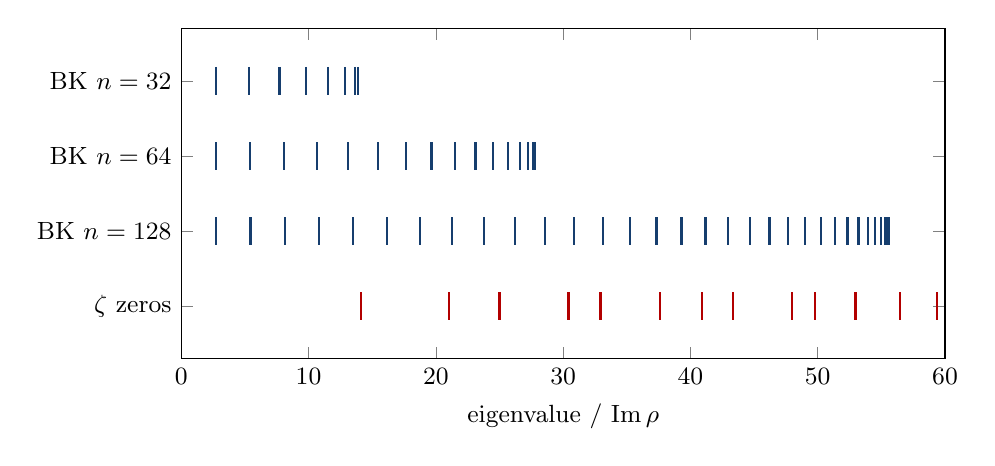
\begin{tikzpicture}
\begin{axis}[scale only axis, width=0.8\linewidth, height=4.2cm, xmin=0, xmax=60, ymin=0.3, ymax=4.7,
  ytick={1,2,3,4}, yticklabels={$\zeta$ zeros, {BK $n=128$}, {BK $n=64$}, {BK $n=32$}},
  xlabel={eigenvalue / $\operatorname{Im}\rho$}, tick label style={font=\small}, label style={font=\small}]
% Generated by paper/figures/make_pgf.sh from the repository data; do not edit.
\addplot[only marks, mark=|, mark size=5pt, thick, color=primary] coordinates { (2.7113,4) (5.3183,4) (7.7210,4) (9.8270,4) (11.5553,4) (12.8395,4) (13.6304,4)
(13.8974,4)};
\addplot[only marks, mark=|, mark size=5pt, thick, color=primary] coordinates { (2.7244,3) (5.4225,3) (8.0684,3) (10.6366,3) (13.1024,3) (15.4420,3) (17.6329,3)
(19.6539,3) (21.4857,3) (23.1106,3) (24.5129,3) (25.6791,3) (26.5980,3) (27.2608,3) (27.6610,3)
(27.7948,3)};
\addplot[only marks, mark=|, mark size=5pt, thick, color=primary] coordinates { (2.7277,2) (5.4487,2) (8.1567,2) (10.8450,2) (13.5072,2) (16.1368,2) (18.7276,2)
(21.2733,2) (23.7677,2) (26.2048,2) (28.5788,2) (30.8840,2) (33.1147,2) (35.2657,2) (37.3318,2)
(39.3078,2) (41.1892,2) (42.9714,2) (44.6501,2) (46.2211,2) (47.6809,2) (49.0257,2) (50.2525,2)
(51.3582,2) (52.3401,2) (53.1960,2) (53.9237,2) (54.5216,2) (54.9880,2) (55.3220,2) (55.5227,2)
(55.5897,2)};
\addplot[only marks, mark=|, mark size=5pt, thick, color=red!70!black] coordinates { (14.1347,1) (21.0220,1) (25.0109,1) (30.4249,1) (32.9351,1) (37.5862,1) (40.9187,1)
(43.3271,1) (48.0052,1) (49.7738,1) (52.9703,1) (56.4462,1) (59.3470,1)};

\end{axis}
\end{tikzpicture}
\caption{Positive eigenvalues of the discretised Berry--Keating operator on $[1,10]$ with $\theta=0$ (each doubly degenerate value drawn once) against the oracle zeros up to $60$. The discrete spectra follow~\eqref{eq:bkspec}: spacing near $2\pi/\ln 10$ at the bottom, compressing towards the band edge $n/\ln 10$. They do not reproduce the zeros.}
\label{fig:bk}
\end{figure}

\begin{remark}
Figure~\ref{fig:bk} is the quantitative form of the statement in the grounding draft: the finite Berry--Keating operator has an arithmetic spectrum, the zeros do not, and no choice of $n$ or $\theta$ changes that. Refining the grid only extends the progression towards the continuum one.
\end{remark}

\section{System Architecture}
\label{sec:arch}

\takeaway{Operating Law}{The model proposes; Fortran and C23 measure; Futhark transforms; OWL classifies; ASP constrains; the proof auditor verifies; and the SHA-256 provenance ledger preserves every decision.}

The original system was written in Python (PyTorch/NumPy/\texttt{mpmath} for measurement, DSPy for conjecture generation, rdflib for the ontology). The native implementation keeps those files as the executable specification and ports each one to the language suited to its layer (Table~\ref{tab:layers}, Figure~\ref{fig:arch}). The native engine has no third-party dependencies: no LAPACK, no BLAS, no JSON or cryptography library.

\begin{table}[!htbp]
\centering
\caption{Architectural layers, responsibilities, and epistemic boundaries in \textsc{Sovereign-RH-Lock}.}
\label{tab:layers}
\begin{tabularx}{\linewidth}{llX}
\toprule
\textbf{Layer} & \textbf{Technology} & \textbf{Core Responsibility \& Epistemic Boundary} \\
\midrule
Conjecture Engine & DSPy / C23 & Ten structured signatures; strict provider temperature validation; bounded provenance DAG (depth 4, branching 3, 64 candidates) with canonical deduplication. \\
Numerical Engine & Fortran 2008 / C23 & Strictly separates $S(\rho) = -\operatorname{Tr}(\rho\log\rho)$, $H(p) = -\sum p_i\log p_i$, and $r(s) = |\zeta(s)|$; $\zeta$ and its zeros in \code{REAL(16)}; Weyl perturbation stability tests. \\
Array Kernels & Futhark / Klong & SoA parallel kernels (\texttt{map}, \texttt{scan}, \texttt{filter}, \texttt{scatter}) over a 32-byte-header + 72-byte/record little-endian 64-bit ABI. \\
Structural Ontology & OWL 2 DL / SWI-Prolog & 15 classes and 9 relations under the Open-World Assumption; enforces disjointness between \texttt{NumericalEvidence} and \texttt{FormalEvidence}; emits ASP facts. \\
Admission Control & Clingo ASP & Closed-world rejection of missing obligations, cyclic proof dependencies and tainted lineages; maintains 5 distinct epistemic states. \\
Formal Layer & Lean 4 / Mathlib & Conditional critical-line theorem, generated lemma families, proof-obligation gates; CI rejects \code{sorry}. \\
\bottomrule
\end{tabularx}
\end{table}

\begin{figure}[!htbp]
\centering
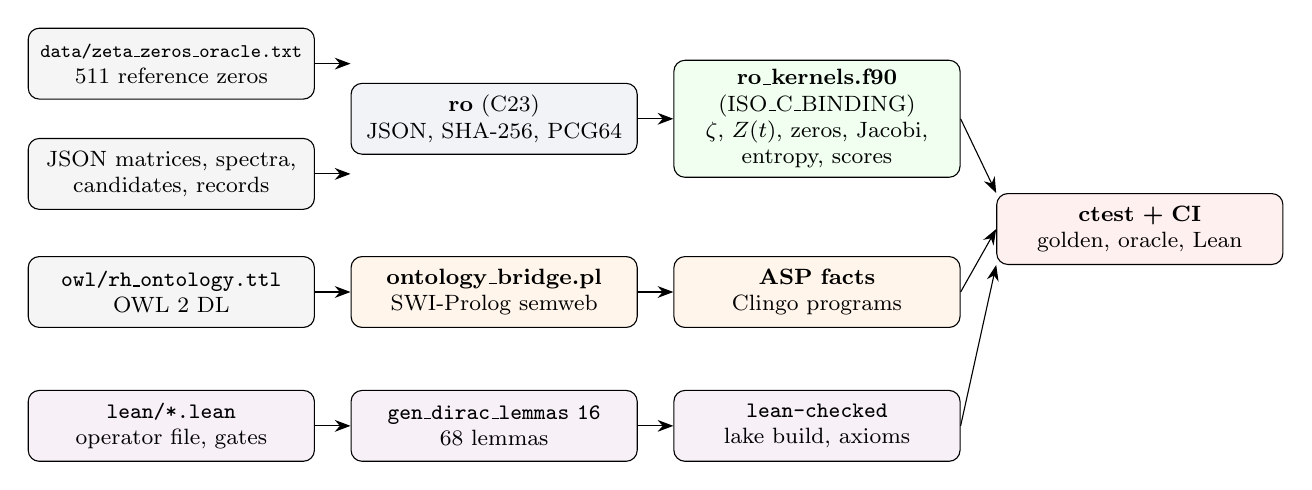
\begin{tikzpicture}[font=\footnotesize,
  box/.style={draw, rounded corners, align=center, minimum height=9mm, text width=34mm, fill=#1},
  box/.default=primary!6, >={Stealth[length=2mm]}]
\node[box=gray!8] (oracle) at (0,0) {{\scriptsize\code{data/zeta\_zeros\_oracle.txt}}\\511 reference zeros};
\node[box=gray!8] (json) at (0,-1.4) {JSON matrices, spectra,\\candidates, records};
\node[box=gray!8] (ttl) at (0,-2.9) {\code{owl/rh\_ontology.ttl}\\OWL 2 DL};
\node[box] (ro) at (4.1,-0.7) {\textbf{ro} (C23)\\JSON, SHA-256, PCG64};
\node[box=green!6] (f90) at (8.2,-0.7) {\textbf{ro\_kernels.f90} (ISO\_C\_BINDING)\\$\zeta$, $Z(t)$, zeros, Jacobi,\\entropy, scores};
\node[box=orange!8] (pl) at (4.1,-2.9) {\textbf{ontology\_bridge.pl}\\SWI-Prolog semweb};
\node[box=orange!8] (asp) at (8.2,-2.9) {\textbf{ASP facts}\\Clingo programs};
\node[box=red!6] (test) at (12.3,-2.1) {\textbf{ctest + CI}\\golden, oracle, Lean};
\node[box=violet!6] (lsrc) at (0,-4.6) {\code{lean/*.lean}\\operator file, gates};
\node[box=violet!6] (gen) at (4.1,-4.6) {\code{gen\_dirac\_lemmas 16}\\68 lemmas};
\node[box=violet!6] (lake) at (8.2,-4.6) {\code{lean-checked}\\lake build, axioms};
\draw[->] (oracle.east) -- (ro.west |- oracle.east); \draw[->] (json.east) -- (ro.west |- json.east);
\draw[->] (ro) -- (f90);
\draw[->] (ttl) -- (pl); \draw[->] (pl) -- (asp);
\draw[->] (f90.east) -- (test.north west); \draw[->] (asp.east) -- (test.west); \draw[->] (lake.east) -- (test.south west);
\draw[->] (lsrc) -- (gen); \draw[->] (gen) -- (lake);
\end{tikzpicture}
\caption{Data flow of the native engine and the formal layer (\code{docs/images/architecture.svg} is the same diagram, generated by \code{docs/plots/architecture.awk}).}
\label{fig:arch}
\end{figure}

\subsection{Ports and their verification}

Table~\ref{tab:ports} lists the Python sources and their ports. The Python files stay in the tree. For every test case the repository stores what the Python printed (\code{tests/golden/}); CI runs only the ports and compares their output with those files. Of the 58 C23/Fortran cases, 49 produce byte-identical output; the other 9 pass through an eigen-solver or a BLAS dot product, where the last bits depend on the order of summation, and agree within the tolerances declared per case in \code{tests/cases.txt}. All 13 Prolog cases are byte-identical. To make byte equality possible the C23 engine writes JSON exactly as Python's \code{json.dumps} does (shortest round-trip float repr, \code{ensure\_ascii}, key sorting), sums like NumPy's pairwise summation, and reproduces \code{numpy.random.default\_rng} bit for bit (SeedSequence, PCG64 and the ziggurat normal sampler).

\begin{table}[!htbp]
\centering
\caption{Python sources and their native ports.}
\label{tab:ports}
\begin{tabularx}{\linewidth}{lX}
\toprule
\textbf{Python} & \textbf{Port} \\
\midrule
\code{torch/spectral.py} & \code{kernels/ro\_kernels.f90} (eigenvalues, $\zeta$, zeros, sums); \code{src/ro\_main.c}; \code{src/ro\_numpy\_rng.c} \\
\code{torch/entropy.py} & \code{ro\_shannon}, \code{ro\_vn\_entropy} (Fortran); \code{shannon}, \code{vn-entropy}, \code{entropy-bounds} (C23) \\
\code{torch/candidates.py} & \code{ro\_priority} (Fortran); \code{rank}, \code{ledger}, \code{pack}, \code{unpack} (C23); \code{src/ro\_sha256.c} \\
\code{dspy/research\_engine.py} & \code{provider}, \code{temp}, \code{lm-config}, \code{provenance}, \code{dag} (C23) \\
\code{dspy/candidate\_optimizer.py} & \code{metric}, \code{select} (C23) \\
\code{dspy/signatures.py} & \code{dspy/signatures.pl} (SWI-Prolog) \\
\code{owl/ontology\_bridge.py} & \code{owl/ontology\_bridge.pl} (SWI-Prolog~\cite{swipl2012}) \\
\bottomrule
\end{tabularx}
\end{table}

\section{Numerical Kernels}
\label{sec:kernels}

\subsection{Zeta in quad precision}
$\zeta(s)$ is evaluated by Euler--Maclaurin summation in Fortran \code{REAL(16)} (IEEE binary128, 113-bit significand):
\begin{equation}
\zeta(s) = \sum_{n=1}^{N-1} n^{-s} + \frac{N^{1-s}}{s-1} + \frac{N^{-s}}{2} + \sum_{k=1}^{M} \frac{B_{2k}}{(2k)!}\, s(s+1)\cdots(s+2k-2)\, N^{-s-2k+1} + R_{N,M},
\end{equation}
with $N = \lfloor |s| \rfloor + 30$ and $M = 36$; the Bernoulli numbers are generated once in \code{REAL(16)} from the recurrence for $B_n/n!$. A double-precision variant ($N = \lfloor |s|/2\rfloor + 12$, $M=12$) is used only to locate sign changes.

\subsection{Hardy's function and the zero finder}
The Riemann--Siegel theta function $\theta(t) = \operatorname{Im}\log\Gamma(\tfrac14 + \tfrac{it}{2}) - \tfrac{t}{2}\log\pi$ is computed in \code{REAL(16)} by Stirling's series after shifting the argument by 24, and Hardy's function is $Z(t) = e^{i\theta(t)}\zeta(\tfrac12+it)$, real for real $t$~\cite{edwards1974,titchmarsh1986}. Zeros are found by scanning $Z$ in double precision from $t=10$ with step $0.02$ and refining every sign change in \code{REAL(16)} by the Illinois variant of regula falsi (the retained endpoint's value is halved when the same side is kept twice), stopping when the bracket is below $10^{-31}$ relative. The $k$-th zero is the $k$-th sign change, so the routine also counts zeros; a missed pair of close zeros would show up as an index mismatch against the oracle.

\subsection{Eigenvalues, entropy and sums}
Hermitian eigenvalues are computed by cyclic Jacobi rotations on the real symmetric $2n\times 2n$ embedding $\begin{psmallmatrix}\operatorname{Re}A & -\operatorname{Im}A\\ \operatorname{Im}A & \operatorname{Re}A\end{psmallmatrix}$, whose eigenvalues are those of $A$, each twice. Shannon entropy $H(p)$ and von Neumann entropy $S(\rho)=-\sum_i \lambda_i\log\lambda_i$ are computed after the same Hermiticity, unit-trace and positivity checks as the Python original; they are never mixed with the zeta residual $r(s)$.

\section{Oracle Verification}
\label{sec:oracle}

\code{data/zeta\_zeros\_oracle.txt} tabulates the imaginary parts of the first 511 nontrivial zeros to ten decimals. \code{ro oracle-check} recomputes every zero with the kernel of Section~\ref{sec:kernels} and requires agreement to the oracle's rounding. The measured result is:
\begin{center}
\begin{tabular}{lr}
\toprule
zeros checked & 511 \\
index or value mismatches & 0 \\
maximum $|t_k^{\mathrm{computed}} - t_k^{\mathrm{oracle}}|$ & $4.99\times 10^{-11}$ \\
maximum $|\zeta(\tfrac12 + it)|$ at the \code{REAL(16)} roots & $1.94\times10^{-28}$ \\
maximum $|\zeta(\tfrac12 + it)|$ at the tabulated (rounded) values & $3.78\times10^{-10}$ \\
wall time (one core) & 16.2 s \\
\bottomrule
\end{tabular}
\end{center}
The deviation is below the oracle's half-unit rounding of $5\times10^{-11}$, and the residual at the tabulated values is of the size expected from that rounding times $|\zeta'|$. The check runs in CI on every push. Independently, the original Python reference, rerun on the benchmark machine with \texttt{mpmath}~1.4.1 at 50 digits, verifies $\rho_1,\dots,\rho_5$ with maximum residual $|\zeta(\rho_k)| = 2.387\times10^{-50}$, and gives $|\zeta(0.6 + i\gamma_1)| = 0.0762$ at an off-line test point, confirming the threshold $|\zeta(0.6+i\gamma_1)|>0.05$ of the grounding draft.

\begin{figure}[!htbp]
\centering
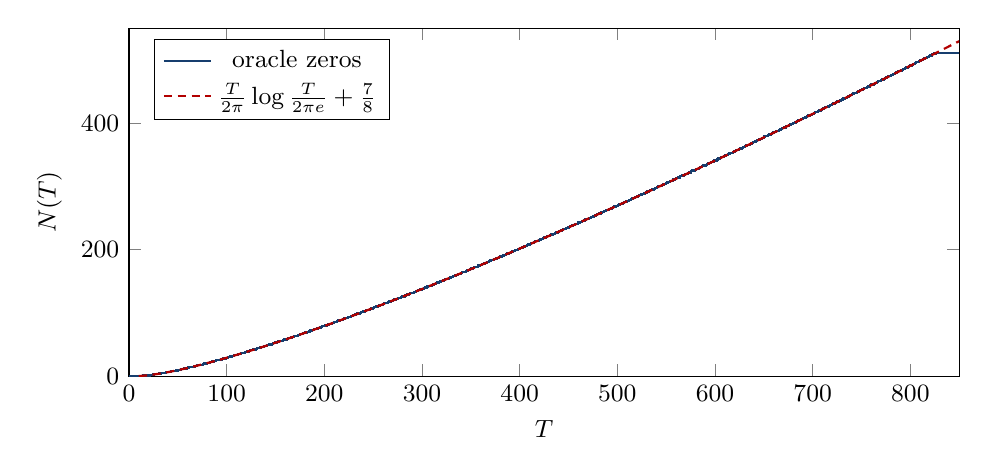
\begin{tikzpicture}
\begin{axis}[width=\linewidth, height=6cm, xmin=0, xmax=850, ymin=0, ymax=550,
  xlabel={$T$}, ylabel={$N(T)$}, legend pos=north west, legend style={font=\small},
  tick label style={font=\small}, label style={font=\small}]
% Generated by paper/figures/make_pgf.sh from the repository data; do not edit.
\addplot[const plot, color=primary, thick] coordinates {(0,0) (14.1347,1) (21.0220,2) (25.0109,3) (30.4249,4) (32.9351,5) (37.5862,6) (40.9187,7)
(43.3271,8) (48.0052,9) (49.7738,10) (52.9703,11) (56.4462,12) (59.3470,13) (60.8318,14) (65.1125,15)
(67.0798,16) (69.5464,17) (72.0672,18) (75.7047,19) (77.1448,20) (79.3374,21) (82.9104,22) (84.7355,23)
(87.4253,24) (88.8091,25) (92.4919,26) (94.6513,27) (95.8706,28) (98.8312,29) (101.3179,30) (103.7255,31)
(105.4466,32) (107.1686,33) (111.0295,34) (111.8747,35) (114.3202,36) (116.2267,37) (118.7908,38) (121.3701,39)
(122.9468,40) (124.2568,41) (127.5167,42) (129.5787,43) (131.0877,44) (133.4977,45) (134.7565,46) (138.1160,47)
(139.7362,48) (141.1237,49) (143.1118,50) (146.0010,51) (147.4228,52) (150.0535,53) (150.9253,54) (153.0247,55)
(156.1129,56) (157.5976,57) (158.8500,58) (161.1890,59) (163.0307,60) (165.5371,61) (167.1844,62) (169.0945,63)
(169.9120,64) (173.4115,65) (174.7542,66) (176.4414,67) (178.3774,68) (179.9165,69) (182.2071,70) (184.8745,71)
(185.5988,72) (187.2289,73) (189.4162,74) (192.0267,75) (193.0797,76) (195.2654,77) (196.8765,78) (198.0153,79)
(201.2648,80) (202.4936,81) (204.1897,82) (205.3947,83) (207.9063,84) (209.5765,85) (211.6909,86) (213.3479,87)
(214.5470,88) (216.1695,89) (219.0676,90) (220.7149,91) (221.4307,92) (224.0070,93) (224.9833,94) (227.4214,95)
(229.3374,96) (231.2502,97) (231.9872,98) (233.6934,99) (236.5242,100) (237.7698,101) (239.5555,102) (241.0492,103)
(242.8233,104) (244.0709,105) (247.1370,106) (248.1020,107) (249.5737,108) (251.0149,109) (253.0700,110) (255.3063,111)
(256.3807,112) (258.6104,113) (259.8744,114) (260.8051,115) (263.5739,116) (265.5579,117) (266.6150,118) (267.9219,119)
(269.9704,120) (271.4941,121) (273.4596,122) (275.5875,123) (276.4520,124) (278.2507,125) (279.2293,126) (282.4651,127)
(283.2112,128) (284.8360,129) (286.6674,130) (287.9119,131) (289.5799,132) (291.8463,133) (293.5584,134) (294.9654,135)
(295.5733,136) (297.9793,137) (299.8403,138) (301.6493,139) (302.6967,140) (304.8644,141) (305.7289,142) (307.2195,143)
(310.1095,144) (311.1651,145) (312.4278,146) (313.9853,147) (315.4756,148) (317.7348,149) (318.8531,150) (321.1601,151)
(322.1446,152) (323.4670,153) (324.8629,154) (327.4439,155) (329.0331,156) (329.9532,157) (331.4745,158) (333.6454,159)
(334.2114,160) (336.8419,161) (338.3400,162) (339.8582,163) (341.0423,164) (342.0549,165) (344.6617,166) (346.3479,167)
(347.2727,168) (349.3163,169) (350.4084,170) (351.8786,171) (353.4889,172) (356.0176,173) (357.1513,174) (357.9527,175)
(359.7438,176) (361.2894,177) (363.3313,178) (364.7360,179) (366.2127,180) (367.9936,181) (368.9684,182) (370.0509,183)
(373.0619,184) (373.8649,185) (375.8259,186) (376.3241,187) (378.4367,188) (379.8730,189) (381.4845,190) (383.4435,191)
(384.9561,192) (385.8613,193) (387.2229,194) (388.8461,195) (391.4561,196) (392.2451,197) (393.4277,198) (395.5829,199)
(396.3819,200) (397.9187,201) (399.9851,202) (401.8392,203) (402.8619,204) (404.2364,205) (405.1344,206) (407.5815,207)
(408.9472,208) (410.5139,209) (411.9723,210) (413.2627,211) (415.0188,212) (415.4552,213) (418.3877,214) (419.8614,215)
(420.6438,216) (422.0767,217) (423.7166,218) (425.0699,219) (427.2088,220) (428.1279,221) (430.3287,222) (431.3013,223)
(432.1386,224) (433.8892,225) (436.1610,226) (437.5817,227) (438.6217,228) (439.9184,229) (441.6832,230) (442.9045,231)
(444.3193,232) (446.8606,233) (447.4417,234) (449.1485,235) (450.1269,236) (451.4033,237) (453.9867,238) (454.9747,239)
(456.3284,240) (457.9039,241) (459.5134,242) (460.0879,243) (462.0654,244) (464.0573,245) (465.6715,246) (466.5703,247)
(467.4390,248) (469.5360,249) (470.7737,250) (472.7992,251) (473.8352,252) (475.6003,253) (476.7690,254) (478.0753,255)
(478.9422,256) (481.8303,257) (482.8348,258) (483.8514,259) (485.5391,260) (486.5287,261) (488.3806,262) (489.6618,263)
(491.3988,264) (493.3144,265) (493.9580,266) (495.3588,267) (496.4297,268) (498.5808,269) (500.3091,270) (501.6044,271)
(502.2763,272) (504.4998,273) (505.4152,274) (506.4642,275) (508.8007,276) (510.2642,277) (511.5623,278) (512.6231,279)
(513.6690,280) (515.4351,281) (517.5897,282) (518.2342,283) (520.1063,284) (521.5252,285) (522.4567,286) (523.9605,287)
(525.0774,288) (527.9036,289) (528.4062,290) (529.8062,291) (530.8669,292) (532.6882,293) (533.7796,294) (535.6643,295)
(537.0698,296) (538.4285,297) (540.2132,298) (540.6314,299) (541.8474,300) (544.3239,301) (545.6368,302) (547.0109,303)
(547.9316,304) (549.4976,305) (550.9700,306) (552.0496,307) (553.7650,308) (555.7920,309) (556.8995,310) (557.5647,311)
(559.3162,312) (560.2408,313) (562.5592,314) (564.1609,315) (564.5061,316) (566.6988,317) (567.7318,318) (568.9240,319)
(570.0511,320) (572.4200,321) (573.6146,322) (575.0939,323) (575.8072,324) (577.0390,325) (579.0988,326) (580.1370,327)
(581.9466,328) (583.2361,329) (584.5617,330) (585.9846,331) (586.7428,332) (588.1397,333) (590.6604,334) (591.7259,335)
(592.5714,336) (593.9747,337) (595.7282,338) (596.3628,339) (598.4931,340) (599.5456,341) (601.6021,342) (602.5792,343)
(603.6256,344) (604.6162,345) (606.3835,346) (608.4132,347) (609.3896,348) (610.8392,349) (611.7742,350) (613.5998,351)
(614.6462,352) (615.5386,353) (618.1128,354) (619.1845,355) (620.2729,356) (621.7093,357) (622.3750,358) (624.2699,359)
(626.0193,360) (627.2684,361) (628.3259,362) (630.4739,363) (630.8058,364) (632.2251,365) (633.5469,366) (635.5238,367)
(637.3972,368) (637.9255,369) (638.9279,370) (640.6948,371) (641.9455,372) (643.2789,373) (644.9906,374) (646.3482,375)
(647.7618,376) (648.7864,377) (650.1975,378) (650.6687,379) (653.6496,380) (654.3019,381) (655.7095,382) (656.9641,383)
(658.1756,384) (659.6638,385) (660.7167,386) (662.2966,387) (664.2446,388) (665.3428,389) (666.5151,390) (667.1485,391)
(668.9758,392) (670.3236,393) (672.4582,394) (673.0436,395) (674.3559,396) (676.1397,397) (677.2302,398) (677.8004,399)
(679.7422,400) (681.8950,401) (682.6027,402) (684.0135,403) (684.9726,404) (686.1632,405) (687.9615,406) (689.3689,407)
(690.4747,408) (692.4517,409) (693.1770,410) (694.5339,411) (695.7263,412) (696.6261,413) (699.1321,414) (700.2967,415)
(701.3017,416) (702.2273,417) (704.0338,418) (705.1258,419) (706.1847,420) (708.2691,421) (709.2296,422) (711.1303,423)
(711.9003,424) (712.7494,425) (714.0828,426) (716.1124,427) (717.4826,428) (718.7428,429) (719.6971,430) (721.3512,431)
(722.2775,432) (723.8458,433) (724.5626,434) (727.0564,435) (728.4055,436) (728.7587,437) (730.4165,438) (731.4174,439)
(732.8181,440) (734.7896,441) (735.7655,442) (737.0529,443) (738.5804,444) (739.9095,445) (740.5738,446) (741.7573,447)
(743.8950,448) (745.3450,449) (746.4993,450) (747.6746,451) (748.2428,452) (750.6560,453) (750.9664,454) (752.8876,455)
(754.3224,456) (755.8393,457) (756.7682,458) (758.1017,459) (758.9002,460) (760.2824,461) (762.7000,462) (763.5931,463)
(764.3075,464) (766.0875,465) (767.2185,466) (768.2815,467) (769.6934,468) (771.0708,469) (772.9616,470) (774.1177,471)
(775.0478,472) (775.9997,473) (777.2997,474) (779.1571,475) (780.3489,476) (782.1377,477) (782.5979,478) (784.2888,479)
(785.7391,480) (786.4611,481) (787.4685,482) (790.0591,483) (790.8316,484) (792.4277,485) (792.8887,486) (794.4838,487)
(795.6066,488) (797.2635,489) (798.7076,490) (799.6543,491) (801.6042,492) (802.5420,493) (803.2431,494) (804.7622,495)
(805.8616,496) (808.1518,497) (809.1978,498) (810.0818,499) (811.1844,500) (812.7711,501) (814.0459,502) (814.8705,503)
(816.7277,504) (818.3807,505) (819.2046,506) (820.7219,507) (821.7135,508) (822.1978,509) (824.5263,510) (826.0393,511) (850,511)};
\addplot[color=red!70!black, densely dashed, thick] coordinates { (10,0.023) (20,1.377) (30,3.565) (40,6.293) (50,9.423) (60,12.873) (70,16.590) (80,20.536) (90,24.680)
(100,29.002) (110,33.484) (120,38.110) (130,42.869) (140,47.750) (150,52.746) (160,57.847) (170,63.048) (180,68.343) (190,73.726)
(200,79.193) (210,84.740) (220,90.362) (230,96.057) (240,101.821) (250,107.651) (260,113.545) (270,119.501) (280,125.515) (290,131.586)
(300,137.712) (310,143.891) (320,150.121) (330,156.401) (340,162.730) (350,169.105) (360,175.526) (370,181.990) (380,188.498) (390,195.048)
(400,201.639) (410,208.269) (420,214.938) (430,221.645) (440,228.389) (450,235.170) (460,241.985) (470,248.836) (480,255.720) (490,262.637)
(500,269.587) (510,276.568) (520,283.581) (530,290.625) (540,297.698) (550,304.801) (560,311.933) (570,319.093) (580,326.281) (590,333.497)
(600,340.739) (610,348.009) (620,355.304) (630,362.625) (640,369.971) (650,377.342) (660,384.738) (670,392.157) (680,399.601) (690,407.067)
(700,414.557) (710,422.070) (720,429.605) (730,437.162) (740,444.741) (750,452.341) (760,459.963) (770,467.606) (780,475.269) (790,482.953)
(800,490.656) (810,498.380) (820,506.124) (830,513.886) (840,521.668) (850,529.469)};

\legend{oracle zeros, $\frac{T}{2\pi}\log\frac{T}{2\pi e} + \frac78$}
\end{axis}
\end{tikzpicture}
\caption{The zero-counting function of the 511 oracle zeros, all at $\sigma=\frac12$, against the Riemann--von Mangoldt main term (\code{docs/images/zeros\_critical\_line.svg} also shows the zeros in the critical strip).}
\label{fig:zeros}
\end{figure}

\section{Spacing Statistics}
\label{sec:gue}

Montgomery's pair-correlation theorem and conjecture~\cite{montgomery1973}, and Odlyzko's computations~\cite{odlyzko1987}, connect the local statistics of the zeros to the Gaussian Unitary Ensemble (GUE). We unfold the oracle zeros with the Riemann--von Mangoldt main term $x(t) = \frac{t}{2\pi}\log\frac{t}{2\pi e} + \frac78$ and normalise the 510 nearest-neighbour spacings by their mean.

\begin{figure}[!htbp]
\centering
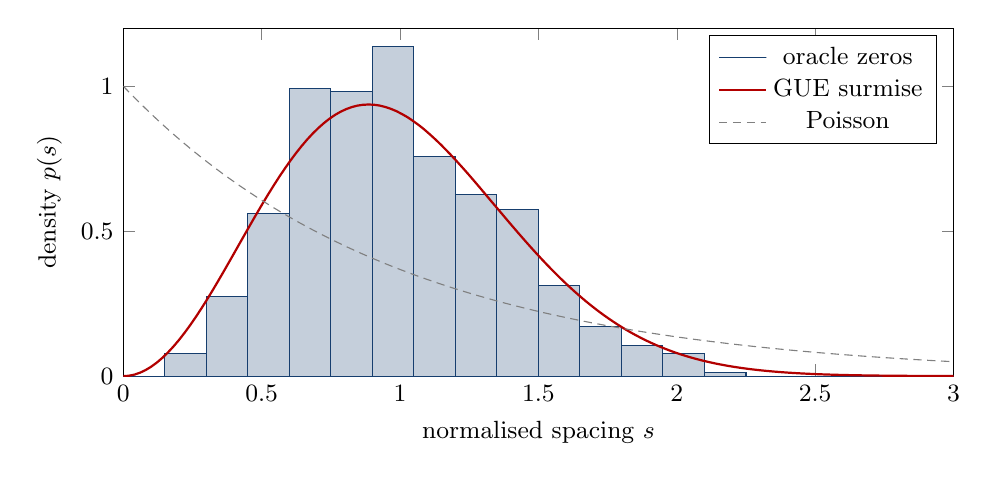
\begin{tikzpicture}
\begin{axis}[width=\linewidth, height=6cm, xmin=0, xmax=3, ymin=0, ymax=1.2,
  xlabel={normalised spacing $s$}, ylabel={density $p(s)$}, legend style={font=\small},
  tick label style={font=\small}, label style={font=\small}]
% Generated by paper/figures/make_pgf.sh from the repository data; do not edit.
\addplot[ybar interval, fill=primary!25, draw=primary] coordinates {
(0.00,0.0000) (0.15,0.0784) (0.30,0.2745) (0.45,0.5621) (0.60,0.9935)
(0.75,0.9804) (0.90,1.1373) (1.05,0.7582) (1.20,0.6275) (1.35,0.5752)
(1.50,0.3137) (1.65,0.1699) (1.80,0.1046) (1.95,0.0784) (2.10,0.0131)
(2.25,0.0000) (2.40,0.0000) (2.55,0.0000) (2.70,0.0000) (2.85,0.0000) (3.00,0)};
\def\spacingcount{510}\def\spacingmean{1.0007}\def\spacingstd{0.3739}

\addplot[domain=0:3, samples=150, thick, red!70!black] {32/pi^2*x^2*exp(-4*x^2/pi)};
\addplot[domain=0:3, samples=100, densely dashed, gray] {exp(-x)};
\legend{oracle zeros, GUE surmise, Poisson}
\end{axis}
\end{tikzpicture}
\caption{Unfolded nearest-neighbour spacings of the oracle zeros (bin width $0.15$) against the GUE Wigner surmise $p(s)=\frac{32}{\pi^2}s^2e^{-4s^2/\pi}$ and the Poisson law $e^{-s}$.}
\label{fig:gue}
\end{figure}

The measured statistics are: mean spacing $1.0007$ before normalisation, standard deviation of the normalised spacings $0.374$ (the GUE surmise has $\sqrt{3\pi/8-1}\approx0.422$, Poisson has $1$), smallest spacing $0.236$, and 3 of 510 spacings below $0.25$. The level repulsion at small $s$ is the qualitative GUE signature; the narrower distribution at these low heights is consistent with Odlyzko's observation that agreement with GUE improves with height~\cite{odlyzko1987}. The discrete Berry--Keating spectra of Section~\ref{sec:bk}, by contrast, have near-constant spacing and no fluctuation at all.

\section{Candidates, Entropy and Provenance}
\label{sec:candidates}

A candidate $C$ carries an entropy $I$, a novelty $N$, an obligation progress $D$ and a residual $R$, and is scored by the heuristic search objective
\begin{equation}
J(C) = w_1 I + w_2 N + w_3 D - w_4 R, \qquad (w_1,w_2,w_3,w_4) = (1.0,\,0.5,\,2.0,\,1.5).
\end{equation}
Ranking sorts by $J$ and then by candidate id, so ties are deterministic. $J$ decides only what to explore next; it never changes an epistemic state. Every candidate, including pruned ones, is appended to a ledger whose entries are the SHA-256 of the compact, key-sorted JSON of the previous hash, the candidate fields and a note, starting from 64 zeros. Arrays of candidates are exchanged in the Klong Structure-of-Arrays format: a 32-byte header \code{"SRHLK64\textbackslash0"}, version, $N$ and column count, followed by nine columns of $N$ little-endian 8-byte values, $32+72N$ bytes in total.

The research engine accepts a model only from a known provider and rejects, rather than clamps, an unsupported temperature. Its provenance DAG is finite by construction: depth at most 4, branching at most 3, at most 64 candidates, with duplicate statements removed after canonicalisation. The ASP layer encodes five mutually distinct epistemic states (candidate, numerically supported hypothesis, formally verified lemma, refuted hypothesis, unresolved conjecture) and the hard constraint that numerical evidence alone can never make a candidate formally admissible; the programs are written for clingo~\cite{clingo2019}.

\section{The Formal Layer in Lean 4}
\label{sec:lean}

The formal layer is a Lake project (\code{lean-checked/}) on Lean~4~\cite{lean4} v4.34.0-rc1 and Mathlib~\cite{mathlib2020} v4.34.0-rc1. The original operator file \code{lean/RiemannDiracOperator.lean} is kept unchanged; \code{RiemannDiracOperator\_checked.lean} is the compiling version.

\subsection{The operator structure and the conditional theorem}

\begin{definition}
A nontrivial zero is $s\in\mathbb{C}$ with \code{riemannZeta s = 0} and $0<\operatorname{Re}s<1$, where \code{riemannZeta} is Mathlib's analytically continued zeta function.
\end{definition}

\begin{definition}
For a complex inner product space $H$, a \code{RiemannDiracOperator H} consists of a continuous linear operator $D$, a proof that $\langle Du,v\rangle=\langle u,Dv\rangle$ for all $u,v$, and a proof of the spectral correspondence: $s$ is a nontrivial zero if and only if $s=\frac12+i\mu$ for an eigenvalue $\mu$ of $D$.
\end{definition}

\begin{theorem}[\code{critical\_line\_of\_dirac\_operator}]
For every $H$, every $D$ of type \code{RiemannDiracOperator H} and every nontrivial zero $s$, $\operatorname{Re}s=\frac12$.
\end{theorem}

The proof uses Mathlib's \code{IsSymmetric.conj\_eigenvalue\_eq\_self} to show that eigenvalues of a symmetric operator are real, and then computes $\operatorname{Re}(\frac12+i\mu)=\frac12$. The theorem is an implication. It does not assert that a \code{RiemannDiracOperator} exists, and constructing one would discharge \texttt{OBL-01} through \texttt{OBL-08} at once. The bounded-operator modelling also departs from the unbounded setting of Section~\ref{sec:bk}: the obligations about domains (\texttt{OBL-02}, \texttt{OBL-04}) have no counterpart in this structure.

\subsection{Recursive lemma generation}

\code{gen\_dirac\_lemmas N} is a command elaborator that recurses on $k=N,N-1,\dots,0$ and, after elaborating level $k-1$, emits four theorems for level $k$: \code{pow\_k\_selfAdjoint} ($D^k$ is self-adjoint, proved from level $k-1$ and the self-adjointness of $D$), \code{pow\_k\_eigenvalue\_real}, \code{pow\_k\_inner\_real} ($\langle D^kv,v\rangle$ is real), and \code{trunc\_k\_nullspace} (a rank-one truncation on $\mathbb{R}^k$ annihilates vectors orthogonal to its right factor). The instance \code{gen\_dirac\_lemmas 16} produces 68 theorems. The closed form \code{selfAdjointRel\_pow}, proved for all $n$ by induction, sits beside them; the generated family is its unfolding to concrete exponents.

\subsection{Axioms}
CI runs \code{\#print axioms} on the main theorems and on the top generated level and fails if \code{sorryAx} appears, and a source scan rejects \code{sorry} and \code{admit}. The measured output is: \code{critical\_line\_of\_dirac\_operator}, \code{all\_nontrivial\_zeros\_on\_line}, \code{selfAdjointRel\_pow} and the four level-16 theorems depend on \code{propext}, \code{Classical.choice} and \code{Quot.sound} only, Lean's standard classical axioms.

\subsection{Lemmas taken from riemann-gas}
The repository \code{AHMADALIPARR/riemann-gas} at commit \code{be609fa} was mined for lemmas that compile against the same Mathlib; each was taken byte for byte with its source noted.
\begin{itemize}
  \item \code{ZetaTruncationProof.lean} compiles whole after moving its import from the nonexistent \code{Mathlib.Basic.Real.Basic} to \code{Mathlib.Data.Real.Basic}: \code{alloy\_red2\_discontinuity} and \code{second\_connector\_fails\_reachability} use no axioms, \code{outer\_product\_nullspace} uses the three standard ones, and the generator reuses it for \code{trunc\_k\_nullspace}.
  \item From \code{DMZ\_F2\_Decomposition.lean}: \code{WeilBound}, \code{weil\_bound\_exists} (no axioms) and \code{weil\_bound\_genus\_two} (by \code{native\_decide}, hence the compiler-trust axiom \code{weil\_bound\_genus\_two.\_native.native\_decide.ax\_1\_1}).
\end{itemize}
The rest of \code{DMZ\_F2\_Decomposition.lean} does not compile, including against the Mathlib revision pinned by its own source project: the import \code{Mathlib.Algebra.BigOperators.Group.Finset} does not exist, and with that path corrected the definitions returning \code{Type*} raise universe errors, \code{MumfordPair.zero} leaves unsolved goals, the operator lemmas on \code{QuantumSpace} (defined locally in the file) fail on missing instances and extensionality, and \code{weil\_bound\_genus\_one} states \code{WeilBound 1 = 7}, which \code{native\_decide} refutes ($\text{WeilBound}(1)=5$). \code{Red2Functor.lean} fails on the unknown constant \code{ZMod.sq\_eq\_self} and a missing \code{HPow}~$\mathbb{C}$~$\mathbb{C}$ instance.

\subsection{Proof-obligation gates in core Lean}
\label{sec:lean-gates}
\code{lean/SovereignRHLock.lean} formalises the audit layer itself using only Lean's core library. It defines the five epistemic states, an obligation status (open, partial, discharged), a ledger with one status per obligation \texttt{OBL-01} to \texttt{OBL-BRIDGE-01}, and the gates as Boolean functions: Gate~9 closes iff \texttt{OBL-04} to \texttt{OBL-07} are discharged, and Gate~10 (RH admission) additionally requires \texttt{OBL-08}. Its seven theorems state that an open Gate~9 blocks Gate~10; that an open \texttt{OBL-06} blocks RH admission; that numerical support and a formally verified lemma are distinct states; that a candidate with a missing obligation is neither retained nor admissible (mirroring \code{proof\_admission.lp}); and three arithmetic facts used by the system: $a<b \Rightarrow \neg(b\le a)$ on $\mathbb{N}$ (named the block-encoding boundedness obstruction), the Klong ABI length $32+9\cdot8n = 32+72n$, and the strict decrease of the remaining search budget. The file compiles unchanged and is built by \code{lean-checked}. Measured axioms: three theorems use none, two use \code{propext}, and the three \code{omega} proofs use \code{propext} and \code{Quot.sound}; CI fails on any other axiom.

\section{Quantum Approach}
\label{sec:quantum}

The quantum track expresses finite truncations of the operator as block encodings in OpenQASM~3.0, on 4 data qubits ($N=16$) and one ancilla.
\begin{itemize}
  \item \code{openqasm/circulant\_qft\_bk.qasm} targets $U_A = (I\otimes F_N^\dagger)\,U_D\,(I\otimes F_N)$, a circulant block encoding meant for the periodic central-difference Berry--Keating stencil of Section~\ref{sec:bk}: a 4-qubit QFT, a diagonal stage of controlled phases with angles $0.25, 0.5, 1, 2$ sandwiched between ancilla Hadamards, and the inverse QFT. Expanded, it applies 10 \code{h}, 20 \code{cp}, 4 \code{swap} and 2 \code{x} gates before measurement.
  \item \code{openqasm/periodic\_diagonal\_lcu.qasm} encodes $D_{\cos}|j\rangle = \cos(\omega j+\phi)|j\rangle$ with $\omega=0.37$, $\phi=0.5$ as a one-ancilla linear combination of $V_{\omega,\phi}$ and $V_{\omega,\phi}^\dagger$, using 2 \code{h}, 2 \code{x}, 2 \code{p} and 8 \code{cp} gates.
\end{itemize}
Both circuits parse without syntax errors under the OpenQASM~3 reference ANTLR grammar (28 and 23 top-level statements). We have not simulated them, so we make no claim here about which matrix each one encodes or about the subnormalisation $\alpha$. Because a block encoding requires $\|A_N\|_2\le\alpha$ and $\|A_N\|_2 = n/\ln(b/a)$ by~\eqref{eq:bkspec}, the subnormalisation grows linearly in $n$: block encodings address finite truncations only, which is the content of the boundedness lemma in Section~\ref{sec:lean-gates}.

\section{Verification Gates and Validation}
\label{sec:gates}

\textsc{Sovereign-RH-Lock} enforces ten sequential verification gates. In this repository they are realised by continuous integration on every push:
\begin{itemize}
  \item \textbf{Native suite (ctest):} 72 tests: 58 golden cases for the Fortran/C23 ports, 13 for the Prolog ports, and the 511-zero oracle check (Section~\ref{sec:oracle}). They cover provider temperature rejection, bounded DAG deduplication, Klong binary round trips, entropy input validation, the ledger and the OWL-to-ASP emission.
  \item \textbf{High-precision spectral check:} the oracle check and the Python reference values of Section~\ref{sec:oracle}; discrete $H_{\mathrm{BK}}$ Hermiticity residual $0.0$; Weyl stability satisfied at $\epsilon=10^{-6}$.
  \item \textbf{Formal build:} \code{lake build} of \code{lean-checked}, the axiom checks of Section~\ref{sec:lean}, and the \code{sorry}/\code{admit} scan.
  \item \textbf{Proof audit:} \textbf{Gate~9} and \textbf{Gate~10} remain \textsc{Open}. \texttt{OBL-04} is \textsc{Partial} (self-adjointness holds for the finite discretisations and is an assumption of the Lean structure, not a theorem about an infinite-dimensional operator), and \texttt{OBL-05} to \texttt{OBL-08} and \texttt{OBL-BRIDGE-01} are \textsc{Open}.
\end{itemize}

\section{Benchmarks}
\label{sec:bench}

Table~\ref{tab:bench} gives median wall times from hyperfine~1.19 (\code{-N}, 3 to 20 runs, with a warm-up run for everything under a minute) on an 8-vCPU Intel Xeon virtual machine running Linux~6.12. The ports were built in Release mode with gcc/gfortran~16.2.0 and SWI-Prolog~10.0.0; the originals ran on Python~3.13.5 with NumPy~2.5.5, \texttt{mpmath}~1.4.1 and rdflib~7.6.0.

\begin{table}[!htbp]
\centering
\caption{Median wall time, native port vs.\ Python original.}
\label{tab:bench}
\begin{tabularx}{\linewidth}{lXrr}
\toprule
\textbf{Task} & \textbf{Input} & \textbf{Port} & \textbf{Python} \\
\midrule
First 511 zeros & \code{ro zeros 511} vs.\ reference loop, $k=1\dots511$ & 15.4 s & 85.5 s \\
One zero & 100th zero, 30 digits & 2.88 s & 0.218 s \\
Hermitian eigenvalues & BK matrix, $n=16$ & 1.4 ms & 99.9 ms \\
 & $n=64$ & 54.6 ms & 98.0 ms \\
 & $n=128$ & 726 ms & 114 ms \\
 & $n=256$ & 11.3 s & 137 ms \\
Von Neumann entropy & $4\times4$ density matrix & 0.7 ms & 69.8 ms \\
Shannon entropy & 10-vector & 0.9 ms & 66.2 ms \\
Candidate ranking & 10\,000 candidates & 132 ms & 141 ms \\
SHA-256 ledger & 10\,000 candidates & 264 ms & 247 ms \\
Ontology check & \code{rh\_ontology.ttl}, 136 triples & 52.7 ms & 133 ms \\
OWL $\to$ ASP facts & \code{rh\_ontology.ttl} & 43.4 ms & 68.9 ms \\
\code{lake build} & \code{lean-checked}, own modules & 7.79 s & --- \\
\bottomrule
\end{tabularx}
\end{table}

Each run is a fresh process, so the Python column includes interpreter start-up and imports (a trivial input takes about 66 ms). The Jacobi solver has no dependencies and falls behind NumPy's LAPACK path past $n\approx100$. A single zero is computed in software \code{REAL(16)} after a scan from $t=10$, which is slower than \texttt{mpmath} at 30 digits; the full scan amortises that cost over all 511 zeros.

\section{Reproducibility}
\label{sec:repro}

All results in this paper come from the repository and can be regenerated with:
\begin{verbatim}
cmake -S . -B build -DCMAKE_BUILD_TYPE=Release -DRO_REQUIRE_PROLOG=ON
cmake --build build -j1 && ctest --test-dir build --output-on-failure
build/ro oracle-check data/zeta_zeros_oracle.txt
cd lean-checked && lake exe cache get && lake build \
  && lake env lean AxiomCheck.lean && lake env lean AxiomCheckSovereign.lean
sh docs/plots/make_figures.sh build/ro      # SVG figures
sh paper/figures/make_pgf.sh build/ro       # data for this paper's plots
\end{verbatim}
The figures in this paper are drawn by pgfplots from coordinate files written by \code{paper/figures/make\_pgf.sh} from \code{data/zeta\_zeros\_oracle.txt} and from \code{ro}; the SVG versions in \code{docs/images/} come from the same data. The Python goldens were produced once from the original sources and are stored as text; the OpenQASM files were checked with the reference grammar in \code{openqasm/openqasm} (\code{source/grammar}) and ANTLR~4.13.2. CI builds this paper on every push.

\section{Conclusion}

\textsc{Sovereign-RH-Lock} turns the Connes--Berry--Keating program into a set of explicit, machine-checked boundaries. The native measurement layer reproduces its Python specification and the 511-zero oracle; the finite Berry--Keating operators are Hermitian but have an arithmetic spectrum given exactly by~\eqref{eq:bkspec}; the zeros themselves repel like GUE eigenvalues; and the Lean layer proves exactly what follows from a self-adjoint operator with the right spectrum, no more. Constructing that operator, the content of \texttt{OBL-01} to \texttt{OBL-08} and \texttt{OBL-BRIDGE-01}, remains open, and the system is built so that it stays recorded as open until it is not.

\begin{thebibliography}{99}
\bibitem{berry1999}
M.~V. Berry and J.~P. Keating, ``The Riemann zeros and eigenvalue asymptotics,'' \emph{SIAM Review}, vol.~41, no.~2, pp.~236--266, 1999.

\bibitem{connes1999}
A.~Connes, ``Trace formula in noncommutative geometry and the zeros of the Riemann zeta function,'' \emph{Selecta Mathematica}, vol.~5, no.~1, pp.~29--106, 1999.

\bibitem{riemann1859}
B.~Riemann, ``Ueber die Anzahl der Primzahlen unter einer gegebenen Gr\"osse,'' \emph{Monatsberichte der K\"oniglich Preu{\ss}ischen Akademie der Wissenschaften zu Berlin}, pp.~671--680, November 1859.

\bibitem{edwards1974}
H.~M. Edwards, \emph{Riemann's Zeta Function}. New York: Academic Press, 1974.

\bibitem{titchmarsh1986}
E.~C. Titchmarsh, \emph{The Theory of the Riemann Zeta-Function}, 2nd ed., revised by D.~R. Heath-Brown. Oxford: Clarendon Press, 1986.

\bibitem{montgomery1973}
H.~L. Montgomery, ``The pair correlation of zeros of the zeta function,'' in \emph{Analytic Number Theory}, Proc.\ Sympos.\ Pure Math., vol.~24. Providence, RI: American Mathematical Society, 1973, pp.~181--193.

\bibitem{odlyzko1987}
A.~M. Odlyzko, ``On the distribution of spacings between zeros of the zeta function,'' \emph{Mathematics of Computation}, vol.~48, no.~177, pp.~273--308, 1987.

\bibitem{lean4}
L.~de~Moura and S.~Ullrich, ``The Lean 4 theorem prover and programming language,'' in \emph{Automated Deduction -- CADE 28}, LNCS vol.~12699. Cham: Springer, 2021, pp.~625--635.

\bibitem{mathlib2020}
The mathlib Community, ``The Lean mathematical library,'' in \emph{Proc.\ 9th ACM SIGPLAN Int.\ Conf.\ on Certified Programs and Proofs (CPP 2020)}. ACM, 2020, pp.~367--381.

\bibitem{swipl2012}
J.~Wielemaker, T.~Schrijvers, M.~Triska and T.~Lager, ``SWI-Prolog,'' \emph{Theory and Practice of Logic Programming}, vol.~12, no.~1--2, pp.~67--96, 2012.

\bibitem{clingo2019}
M.~Gebser, R.~Kaminski, B.~Kaufmann and T.~Schaub, ``Multi-shot ASP solving with clingo,'' \emph{Theory and Practice of Logic Programming}, vol.~19, no.~1, pp.~27--82, 2019.
\end{thebibliography}

\end{document}
